\documentclass[12pt]{article}
\usepackage{graphicx, amsmath}
\usepackage{caption}
\usepackage{algorithm}
\usepackage{algpseudocode}
\graphicspath{ {./} }
\setlength{\oddsidemargin}{0.25 in}
\setlength{\evensidemargin}{-0.25 in}
\setlength{\topmargin}{-0.6 in}
\setlength{\textwidth}{6.5 in}
\setlength{\textheight}{8.5 in}
\setlength{\headsep}{0.75 in}
\setlength{\parindent}{0 in}
\setlength{\parskip}{0.1 in}

\begin{document}
\thispagestyle{plain}
   \newpage
   \setcounter{page}{1}
   \noindent
   \begin{center}
   \framebox{
      \vbox{\vspace{2mm}
    \hbox to 6.28in { {\bf BioE 131: Intro to Computational Biology}
                        \hfill Fall 2020 }
       \vspace{4mm}
       \hbox to 6.28in { {\bf \Large \hfill Phylogeny  \hfill} }
       \vspace{2mm}
       \hbox to 6.28in { {\it Professor: Ian Holmes \hfill} }
      \vspace{2mm}}
   }
   \end{center}
   {Notes written by Vikram Shivakumar}
   \vspace*{4mm}


\section{Introduction}
Often, multiple alignments are constructed with the ultimate goal of studying the relationships between sequences (and species), which we can visualize using \textbf{Phylogenetic trees}. In this note, we will explore methods for building and analyzing phylogenies, as well as the Jukes-Cantor model for estimating evolution distance.
\section{fUn WiTh GrApHs}
Phylogenetic trees (or dendograms, or cladograms), like all trees, are special types of \textbf{graphs}. Graphs are a set of \textbf{vertices} (or \textbf{nodes}),   connected by \textbf{edges}. Edges can be \textbf{directed} or \textbf{undirected}, as well as labeled with weights or distances. The node \textbf{degree} is the number of neighbors of the node (for directed graphs, each node has an in-degree and out-degree).
\begin{figure}[h]
    \centering
    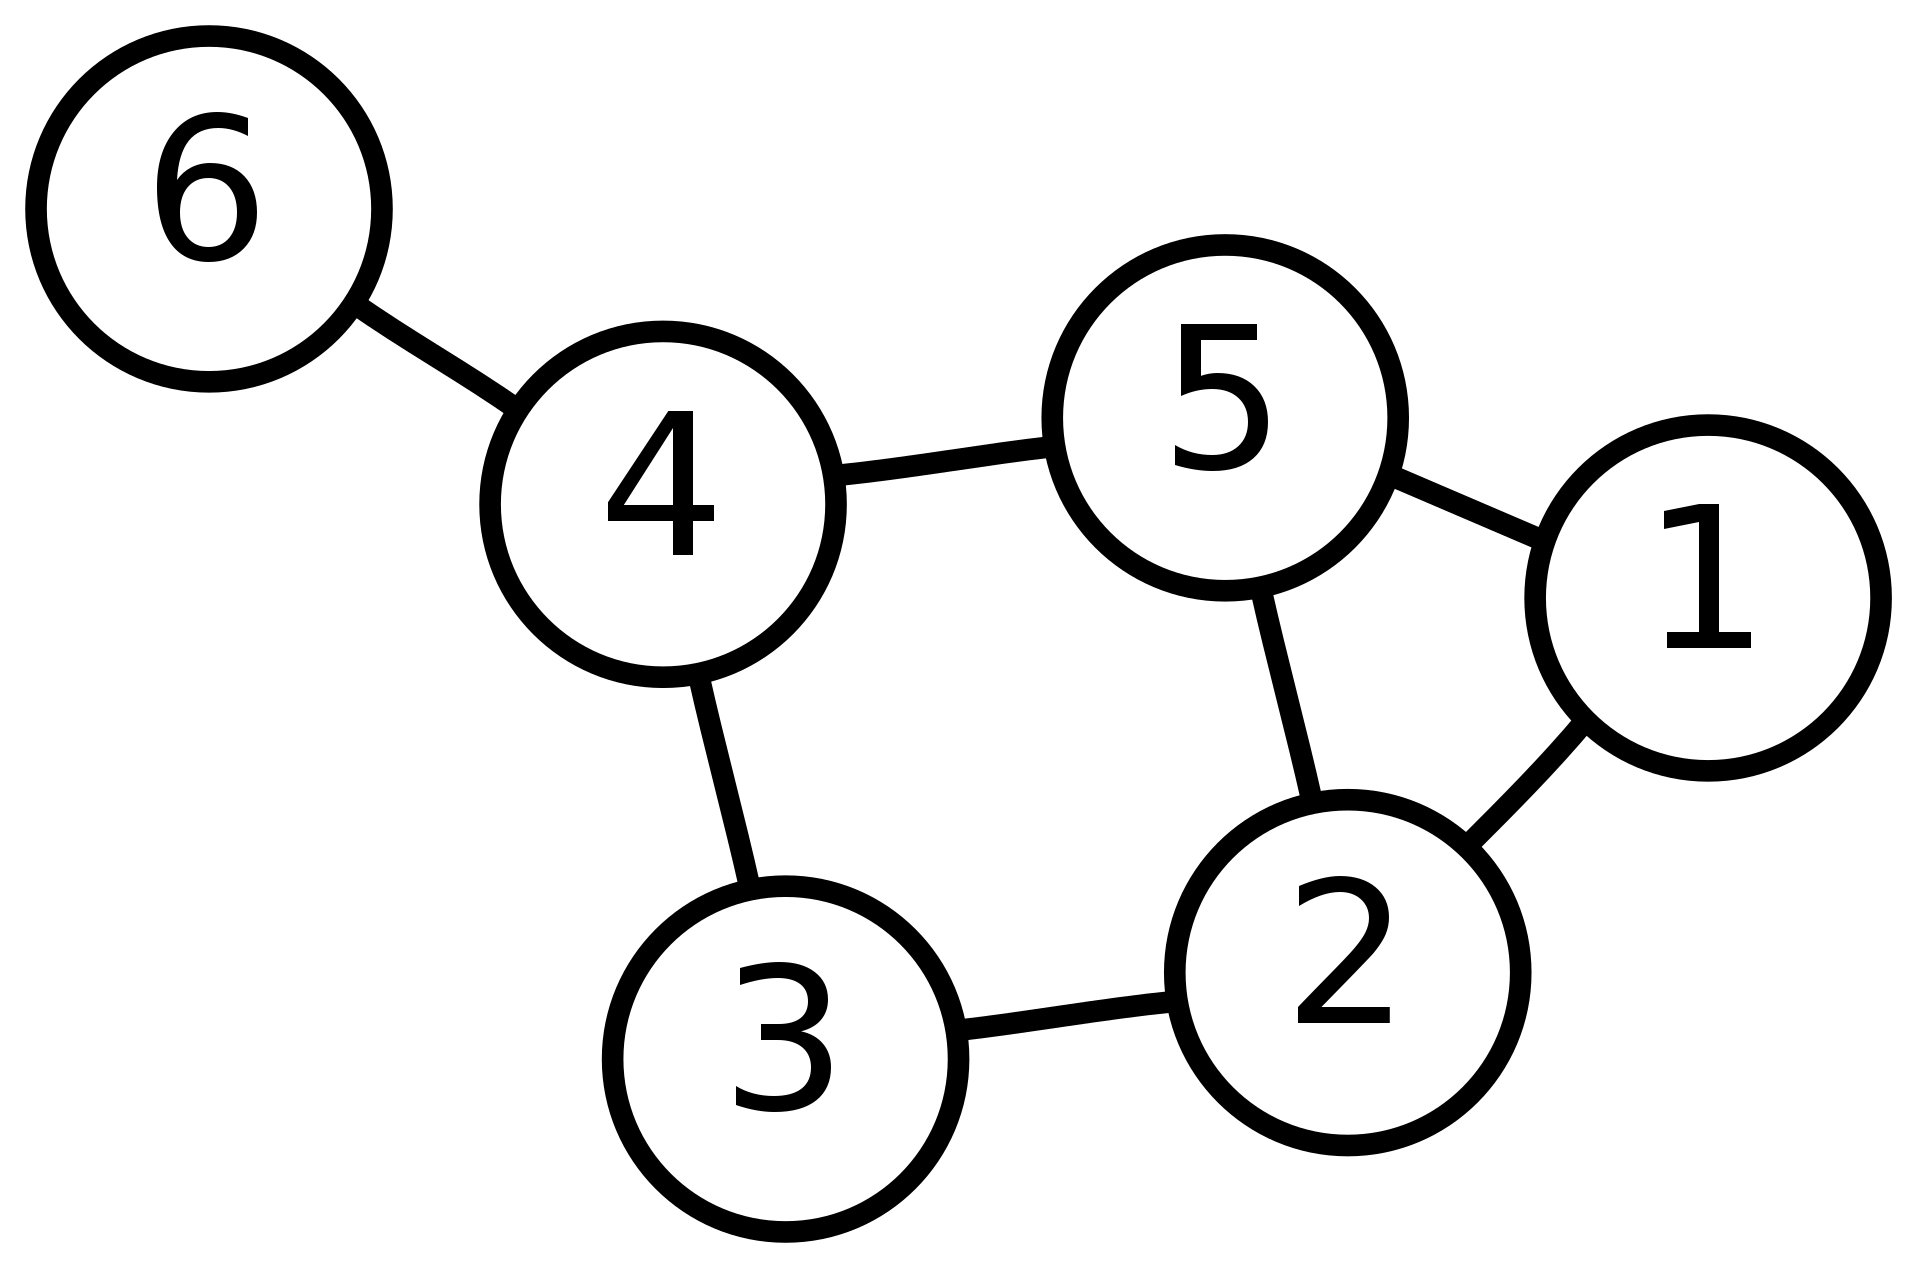
\includegraphics[width=.4\linewidth]{graph.png}
    \caption{Example of an undirected cyclic graph with 6 vertices}
    \label{fig:graph}
\end{figure}
Graphs can be \textbf{connected}, if there is a \textit{path} between any two vertices. They can also be \textbf{complete}, if there is an edge between every pair of vertices. Lastly, graphs can be \textbf{acyclic} if there are no cycles (a path from a vertex to itself).\\[10pt]
A tree is a special type of graph that is connected and acyclic. Trees are also \textbf{minimally connected}, with exactly $|V| - 1$ edges, where $|V|$ is the number of vertices.  A \textbf{binary tree} is a tree where all nodes are internal (degree 3), leaves (degree 1), or the root (degree 2). Phylogenetic trees had edge labels (representing evolutionary distances), and node labels (gene or taxons). Lastly, a root node is specified, which implies directionality in the graph (edges are directed \textit{away} from the root).

\section{Phylogenetic Trees}
Phylogenetic trees are often rooted such that the tree is directed. In phylogenies of taxons, the root represents a common ancestor of the leaf nodes, and in phylogenies of genes, the root node represents the \textbf{ancestral sequence}. \textbf{Outgroups}, species which are distantly related to the rest of the tree, can be included to root the tree. Often times the root can be ambiguous, e.g in the tree of life, there is no outgroup to determine the root.\\[10pt]
\begin{figure}[h]
    \centering
    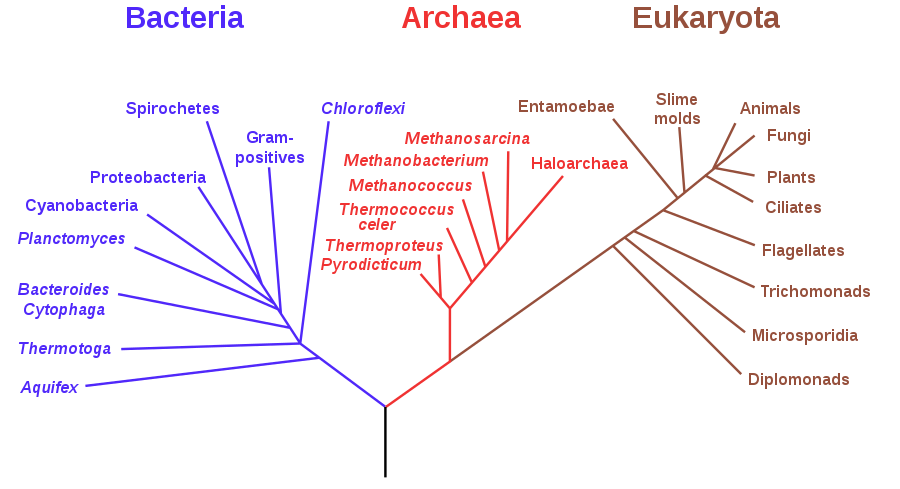
\includegraphics[width=.6\linewidth]{tree_of_life_rooted.png}
    \caption{Tree of life with a possible root (between Bacteria and Archeae)}
    \label{fig:life}
\end{figure}\\[10pt]
Lastly, trees can be \textbf{ultrametric}, where the leaf nodes are the same distance from the root. 
One example of an ultrametric tree is from the \textbf{coalescent process}, which models running time backwards in the Wright Fisher Model (see the note on Probability). Non-ultrametric trees can result from data where the leaf nodes are not contemporaneous (e.g. sequencing ancient DNA). Branch lengths can also vary between contemporaneous taxa, where factors like metabolic rate and mutation rate vary.
\begin{figure}[h]
    \centering
    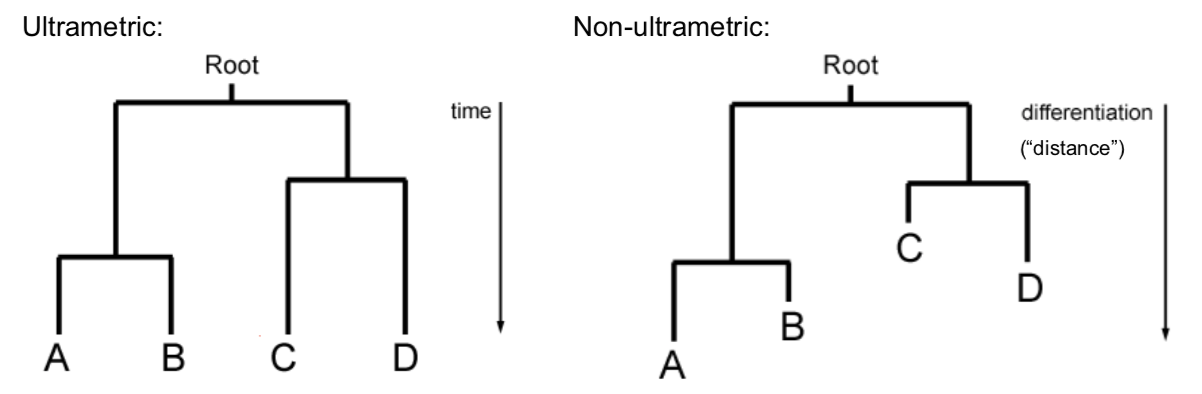
\includegraphics[width=.85\linewidth]{ultrametric.png}
    \caption{Ultrametric vs Non-ultrametric trees}
    \label{fig:ultra}
\end{figure}

\section{Algorithms for Phylogenetic Reconstruction}
Now let's look at a few methods to construct phylogenetic trees from multiple alignments. In general, the substitutions (and in some cases the indels) in the MSA are used to build and evaluate a tree.
\subsection{Parsimony}
\textbf{Parsimony trees} group taxa such that the number of substitutions is minimized. These trees are the simplest type of phylogenetic trees, and can be solved using various optimization methods (like the \textbf{branch-and-bound} method). However, this method ignores different types of substitutions, treating them all the same. It also does not account for \textbf{back-substitutions}, where a mutation reverts a previous mutation (and the final nucleotide appears unchanged).
\subsection{Distance Matrix}
We can also construct a phylogeny (or any distance tree) from a \textbf{distance matrix}, which contains the ``distance" between each taxon or gene. This works well if distances are \textbf{additive} (not the case with back-substitutions!). This method can be a quick approximation for likelihood methods (which we will explore later), but can be prone to certain types of error.\\[10pt] One type of error is \textbf{long branch attraction}. When two species are on long branches in a phylogenetic tree, there can be chance similarities due to a long time to accumulate sequence or morphological changes. This can cause distantly related species to appear more related!
\subsubsection{UPGMA algorithm}
Using a multiple alignment, we can build a matrix of pairwise distances, and construct an ultrametric tree using the \textbf{UPGMA} algorithm.\\[10pt]
The general idea of the algorithm is:
\begin{enumerate}
    \item Pick the closest two nodes, and group them under an ancestral node
    \item The distance between \textbf{ancestral nodes} is the average over the distances between all descendents
    \item Repeat until all nodes are included
\end{enumerate}
We can describe the UPGMA algorithm in pseudo-code:
\begin{algorithm}
\caption{UPGMA algorithm}
\hspace*{\algorithmicindent} \textbf{Input}: Distance matrix, $D_{ij}$
\begin{algorithmic}
\State Let $N$ be a set of nodes
\State Let $C(i)$ be the set of descendants of node $i$
\For{nodes $\in N$}
    \State$C(i) \leftarrow \{i\}$
\EndFor
\While{$N$ contains nodes}
    \State $(i, j) \leftarrow \arg\min_{i,j}D_{i,j}$
    \State Create node $k$
    \State $C(k) \leftarrow C(i) \bigcup C(j)$
    \For{nodes $\in N$}
        \State $D_{kn} \leftarrow \langle D_{xy}\rangle_{x\in C(k), y\in C(n)}$
    \EndFor
\EndWhile
\end{algorithmic}
\end{algorithm}
\subsubsection{Runtime Complexity of UPGMA}
Looking at the pseudocode, the initialization takes $O(N-1)$ steps. The \textit{while} loop runs in $O(N)$ time, and in each loop, we find the smallest item in the matrix $D$, which naively takes $O(N^2)$ time (though this can be reduced by storing the smallest value). Thus the while loop takes $O(N^3)$ time, which is the overall runtime of the algorithm. The memory complexity is simply $O(N^2)$, since the algorithm stores the distance matrix in memory.

\subsection{Phylogenetic Likelihood}
Phylogenetic likelihood methods for tree construction find the tree with the most likely substitutions. These trees are more realistic than those from distance matrix or parsimony approaches, but they can be much slower, as they evaluate the likelihood of many tree topologies.
\begin{figure}[h]
    \centering
    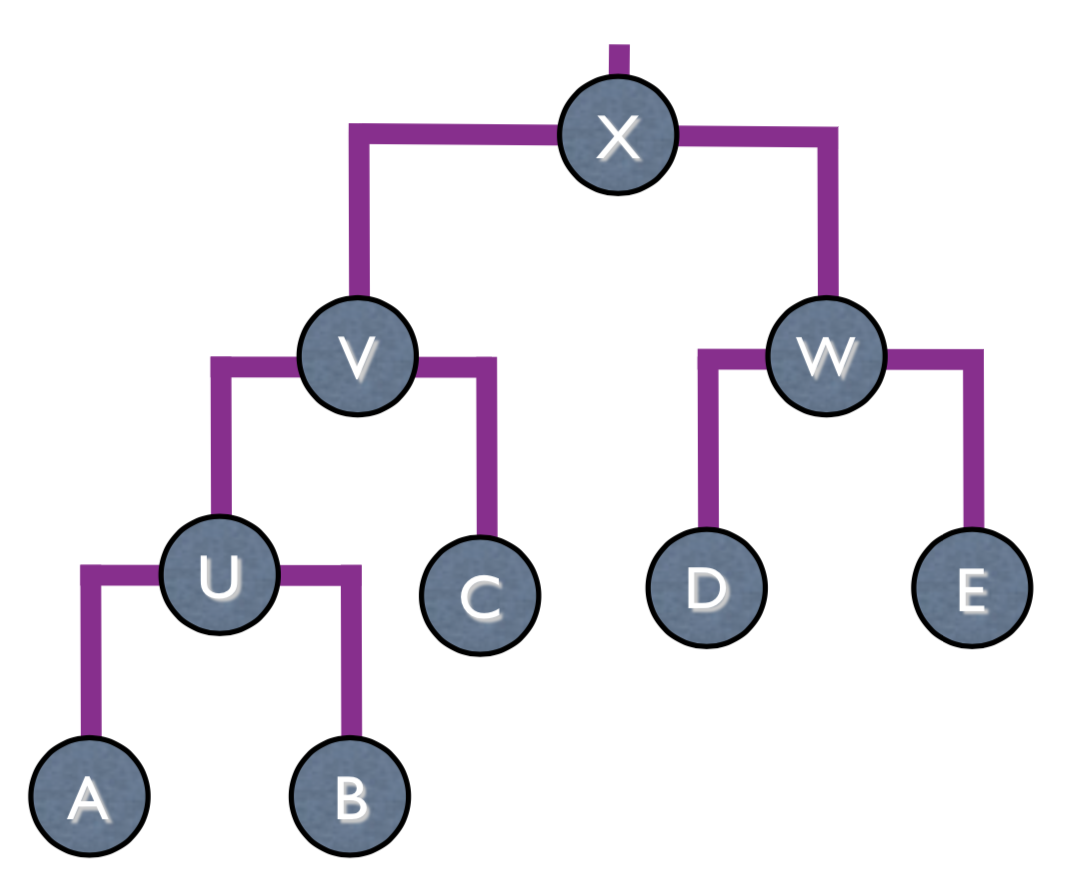
\includegraphics[width=.5\linewidth]{tree.png}
    \caption{Example of a phylogenetic tree}
    \label{fig:tree}
\end{figure}
\subsubsection{Likelihood}
We can calculate the likelihood of a tree using the probability distribution over the root $P(x)$, and the conditional distribution of a node, $P(w|x)$, the probability of a node given its parent. Thus for the tree in Figure \ref{fig:tree}, the likelihood would be:
$$L_0 = P(x) \cdot P(v|x) \cdot P(u|v) \cdot P(a|u) \cdot P(b|u) \cdot P(c|v) \cdot P(w|x) \cdot P(d|w) \cdot P(e|w)$$
However, we don't knnow the ancestral states (in this case nodes $u, v, w, $ and $x$). Thus we can sum over all possible states of these nodes.
$$L = \sum_u\sum_v\sum_w\sum_xL_0$$
Since there are order $O(N)$ internal nodes in a tree, iterating through all possible states for all ancestral nodes would take $O(A^N)$ times ($A$ is the alphabet size, e.g. 4 for nucleotide sequences).\\[10pt]
We can use dynamic programming to reduce the runtime to $O(A^2N)$! The idea is to compute the likehood of each subtree, and recursively calculate the final likelihood. This is equivalent to rearranging the likelihood sum:
$$\sum_x P(x) \left(\sum_v P(v|x)\left(\sum_u P(u|v) \cdot P(a|u) \cdot P(b|u)\right) P(x|v) \right)\left(\sum_w P(w|x)\cdot P(d|w) \cdot P(e|w)\right)$$
Now, each sum represents sum in parantheses represents a partial solution $P(\text{subtree} | \text{root})$.
\subsubsection{Confidence estimates}
Often phylogenies include the confidence of branches, which can be determined directly from likelihood methods (like MCMC sampling), or by \textbf{bootstrapping}. Bootstrapping involves sampling a random set of columns from the multiple alignment (\textit{with} replacement), and building a tree from just that subset of data. We can repeat this many times, and find the percent of trees which include a certain branch in their topology. 

\subsubsection{Other methods}
Other algorithms have been developed to build phylogenies from multiple alignments, which approximate likelihood methods. \textbf{Neighbor-joining} is an algorithm that extends the ideas from UPGMA, but allows for siblings to be non-equidistant from the parent. Thus, neighbor-joining methods can also produce non-ultrametric trees. \textbf{Weighted neighbor-joining} improves on normal neigbor-joining by correcting for long-branch estimation error. \textbf{Quartet-puzzling} algorithms look at sets of 4 nodes in the tree, and finds the best arrangement for each local set of 4, as opposed to comparing pairs of nodes \\[10pt]
Lastly, \textbf{MCMC sampling} is an important algorithm for approximating the likelihood of a tree. This method stochastically generates trees from the underlying probability distribution of trees, which (after enough trees have been generated) can be used to calculate the probabilities of each tree. This method is slow, but the longer it runs, the more accurate an approximation to the maximum likelihood tree it can provide.

\section{Jukes Cantor Model}
The Jukes Cantor model was developed at Berkeley in 1969 as a method to estimate evolutionary distances between sequences. We'll derive the equation for the distance estimate in this section.\\[10pt]
Let's assume in a sequence, there are randomly timed replacement events, where a nucleotide is replaced by any of the 4 nucleotides with uniform probability (so there is a 1/4 probability of the nucleotide remaining the same). We can model these replacements with a \textbf{Poisson} distribution, with a mean of $RT$, where $R$ is the rate of replacement events, and $T$ is time. \textit{Note}: the rate of \textit{substitutions} is $\lambda = \frac{3}{4}R$.\\[10pt]
Now let $X(t)$ be the state of the process at time $t$, and $Q(t)$ be the probability that there are \textit{no replacements} from time $0$ to $t$. Since $R$ is the rate of replacement events, we can derive an expression for $Q(t)$:
\begin{equation}
    \frac{dQ}{dt} = -RQ
\end{equation}
Since $Q(0) = 1$, we can solve the differential equation:
\begin{equation}
    Q(t) = \exp(-Rt)
\end{equation}
Now let's find the probability that the state of the process at time $t$ is the same as the initial state, i.e. $P\left(X\left(t\right) = X\left(0\right)\right)$. If the state of the process remains the same, then there were EITHER no replacement events in time $t$ OR the replacements did not change the nucleotide (with probability 1/4):
\begin{equation}
    P\left(X\left(t\right) = X\left(0\right)\right) = Q\left(t\right) + \frac{1-Q\left(t\right)}{4}
\end{equation}
We can further simplify this equation:
\begin{equation}
    P\left(X\left(t\right) = X\left(0\right)\right) = \frac{1}{4}\left(1 + 3\exp\left(-Rt\right)\right)
\end{equation}
Now let's look at a pairwise alignment of two sequences with length $L$. Assume the sequences are seperated by \textbf{evolutionary distance} $t$. If we assume that each nucleotide is independent, then we can find the \textbf{expected number of matches} $M$ (same nucleotide in both sequences at a position):
\begin{equation}
    M = L \times \frac{1}{4}\left(1 + 3\exp\left(-Rt\right)\right)
    \label{matches}
\end{equation}
But we are trying to find an equation to estimate the evolutionary distance $t$! Let's rearrange equation (\ref{matches}) to find $t$:
\begin{equation}
    t = -\frac{1}{R} \log \left(\frac{1}{3}\left(4\frac{M}{L} - 1 \right)\right)
    \label{calc_t}
\end{equation}
Lastly, we can calibrate time such that the rate of substitutions is 1, i.e. $\lambda = 1$, which implies that the rate of replacement $R = \frac{4}{3}$. We can plug in this rate to derive the full Jukes-Cantor distance estimate:
\begin{equation}
    t = -\frac{3}{4} \log \left(\frac{4}{3}\frac{M}{L} - \frac{1}{3} \right)
    \label{final_jc}
\end{equation}
We can also rewrite this equation in terms of the number of \textit{mismatches} instead of matches, $q = 1-M/L$:
\begin{equation}
    t = -\frac{3}{4} \log \left(1 - \frac{4}{3}q \right)
    \label{jukesbox_hero}
\end{equation}

\section{Virus design}
One problem in bioinformatics is designing therapeutic viruses for various purposes like delivering genetic material or lysing specific cells. These designed viruses need to have a few properties, like safety (not involved in disease), stability, and ease of transformation. Another property that is important, related to evolution, is the rate of \textbf{nonsynonymous mutations}. These mutations change the amino acid sequence of the expressed protein, unlike \textbf{synonymous mutations}, which are silent, and cause no change in the overall protein sequence. One common metric to calculate is the \textbf{Ka/Ks ratio}, or the dN/ds ratio. This is the ratio of nonsynonymous to synonymous mutations, and can reveal information about the selective pressures driving evolution of the gene (or in this case, viral genome). There are ranges of values for the ratio:
\begin{enumerate}
    \item Ka/Ks $>1$: \textbf{diversifying selection}, the case in pathogens undergoing immune system evasion
    \item Ka/Ks $\approx 1$: \textbf{neutral selection}
    \item Ka/Ks $< 1$: \textbf{purifying selection}, such as in the case of housekeeping genes
\end{enumerate}
By measuring the Ka/Ks ratio of a virus, we can study the selective evolutionary pressures that a virus is undergoing, and better understand how viruses evolve.

\section{Summary}
Phylogenetic trees are an important tool to understand the evolutionary relationships between taxa or sequences. We can used properties of graphs to study phylogenies, and reconstruct trees using various methods. We can also use probabilistic models like the Jukes-Cantor model to estimate the evolutionary distance between sequences. Lastly, evolutionary models can be useful in the study of viruses, which undergo selective pressures that drive genetic change.



\end{document}


%topics not covered:
%star vs hierarchal phylogenies
%long-branch attraction
%extra jukes cantor, 241 material